\begin{savequote}[45mm]
\ascii{Any fool can write code that a computer can understand. Good programmers write code that humans can understand.}
\qauthor{\ascii{- Martin Flower}}
\end{savequote}

\chapter{破冰之旅} 
\label{ch:ice-breaker}

\begin{content}

\end{content}

\section{编程环境}

\begin{content}

\subsection{系统配置}

\begin{table}[!htb]
\resizebox{0.8\textwidth}{!} {
\begin{tabular*}{1.2\textwidth}{@{}ll@{}}
\toprule
\ascii{环境} & \ascii{配置与版本} \\
\midrule
\ascii{操作系统}  & \ascii{Ubuntu 18.04} \\
\ascii{编译器} & \ascii{GCC 7.3.0} \\ 
\ascii{编程语言} & \ascii{C++14} \\ 
\ascii{构建工具} & \ascii{CMake 3.10, Make 4.1} \\ 
\ascii{集成开发环境} & \ascii{Eclipse CDT Oxygen.3} \\ 
\bottomrule
\end{tabular*}
}
\caption{环境配置}
\label{tbl:env-configure}
\end{table}

\subsection{项目组织}

\ascii{xUnit Mars}项目物理目录结构如下所示。

\begin{leftbar}
 \begin{c++}[caption={\ttfamily{项目组织}}]
mars
├── build
├── CMakeLists.txt
├── include
│   └── mars
├── src
│   ├── CMakeLists.txt
│   └── mars
└── test
    ├── CMakeLists.txt
    └── mars
 \end{c++}
\end{leftbar}

\subsection{构建系统}

\ascii{xUnit Mars}使用\ascii{CMake}构建工具。在项目根目录下,主控\ascii{CMakeLists.txt}完成项目的整体配置,及其子任务的组织。

\begin{leftbar}
 \begin{c++}[caption={\ttfamily{CMakeLists.txt}}]
project(mars)                                                                                  
cmake_minimum_required(VERSION 2.8)

set(CMAKE_CXX_FLAGS "${CMAKE_CXX_FLAGS} -std=c++14")

include_directories("${CMAKE_CURRENT_SOURCE_DIR}/include")

add_subdirectory(src)
add_subdirectory(test)
 \end{c++}
\end{leftbar}

\ascii{src/CMakeLists.txt}完成\ascii{mars}库构建。

\begin{leftbar}
 \begin{c++}[caption={\ttfamily{src/CMakeLists.txt}}]
file(GLOB_RECURSE all_files *.cc)
add_library(mars STATIC ${all_files})
 \end{c++}
\end{leftbar}

\ascii{test/CMakeLists.txt}完成\ascii{mars-test}应用程序构建,它执行\ascii{xUnit Mars}项目的所有测试用例。

\begin{leftbar}
 \begin{c++}[caption={\ttfamily{test/CMakeLists.txt}}]
file(GLOB_RECURSE all_files *.cc)
add_executable(mars-test ${all_files})
target_link_libraries(mars-test mars gtest gtest_main pthread)
 \end{c++}
\end{leftbar}

\subsection{Git库}

在项目根目录下初始化一个空的\ascii{Git}库。

\begin{leftbar}
 \begin{c++}[caption={\ttfamily{初始化git库}}] 
$ git init
 \end{c++}
\end{leftbar}  

待项目组织完毕,完成第一次代码提交。

\begin{leftbar}
 \begin{c++}[caption={\ttfamily{提交代码}}] 
$ git add -A .
$ git commit -m"setup project"
 \end{c++}
\end{leftbar}

\end{content}

\section{起航}

\begin{content}

\subsection{测试用例}

万事开头难,第一个用例跑起来并不容易。此处设计实现了一个简单的测试用例,用户通过扩展\ascii{xUnit Mars}框架中的\ascii{TestCase},增加新的测试用例。一般地,在面向对象设计中,扩展子类实现是遵循开放封闭原则的重要手段。

\begin{leftbar}
 \begin{c++}[caption={\ttfamily{test/mars/core/TestCaseSpec.cc}}]
#include <gtest/gtest.h>
#include "mars/core/TestCase.h"

namespace {
  struct SimpleTest : TestCase {
    bool wasRun = false;

  private:
    void run() override {
      wasRun = true;
    }
  };

  void run(TestCase& test) {
    test.run();
  }
}

TEST(SimpleTest, make_sure_test_case_can_run_normally) {
  SimpleTest test;
  run(test);

  ASSERT_TRUE(test.wasRun);
}
 \end{c++}
\end{leftbar}

\begin{episode}{TDD: 测试驱动开发}

\begin{content}

\ascii{TDD}是极限编程中重要的技术实践之一。\ascii{TDD}遵循小步快走,测试先行的基本方法论,每轮迭代依次执行\ascii{“Red-Green-Refactor”};每轮迭代之后,系统都处于一个相对合理的状态,如\refig{tdd-cycle}所示。

\begin{figure}[H]
\centering
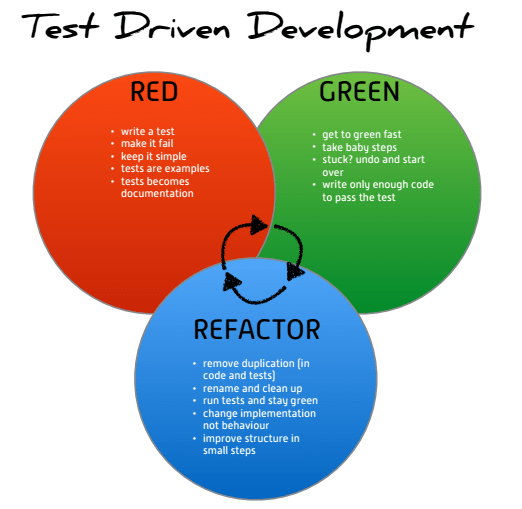
\includegraphics[width=0.8\textwidth]{figures/xunit/tdd_cycle.png}
\caption{TDD环}
 \label{fig:tdd-cycle}
\end{figure}

\end{content}

\end{episode}

\subsection{通过编译}

此处引入了多态技术,当\ascii{TestCase::run}启动运行时,将在运行时调用覆写的\ascii{SimpleTest::run},实现自定义测试用例的执行。

\begin{leftbar}
 \begin{c++}[caption={\ttfamily{include/mars/core/TestCase.h}}]
#ifndef H586108AA_CD7B_459D_8A2F_0DFE6C9720ED
#define H586108AA_CD7B_459D_8A2F_0DFE6C9720ED

struct TestCase {
  virtual ~TestCase() {}
  virtual void run() = 0;
};

#endif
  \end{c++}
\end{leftbar}


\begin{episode}{头文件保护宏}

\begin{content}

\ascii{C/C++}的编译模型通过使用\ascii{include}语句载入头文件,为了避免头文件被载入多次,每一个头文件都应该定义独一无二的头文件保护宏,社区存在两种风格:

\begin{enum}
  \eitem{\code{INCL\_<PROJECT>\_<MODULE>\_<FILE>\_H}}
  \eitem{\ascii{UUID}}
\end{enum}

第一种命名风格问题在于:当头文件被重命名或移动目录时,为了保持一致性需要同步修改头文件保护宏,而此特性\ascii{IDE}通常支持都不是太良好。因此,推荐使用\ascii{IDE}自动地随机生成\ascii{UUID},其更加快捷、简单、并且安全、有效。

其中,\ascii{Eclipse CDT}使用代码模板,并执行如下配置,创建头文件时自动生成\ascii{UUID}的头文件保护宏。

\begin{leftbar}
 \begin{c++}[caption={\ttfamily{头文件保护宏:配置Eclipse CDT生成UUID}}]
$ vi .settings/org.eclipse.cdt.ui.prefs
codetemplates.includeGuardGenerationScheme=1    
eclipse.preferences.version=1
formatter_settings_version=1
 \end{c++}
\end{leftbar}

为了缩短篇幅,后文略去所有头文件保护符。

\end{content}

\end{episode}

需要重点关注的是,\ascii{TestCase}显式地声明了虚拟的析构函数。如果不经意地遗忘声明该析构函数为虚拟的,则可能招致运行时不确定的行为发生。

\begin{episode}{析构函数:虚拟 VS. 非虚}

\begin{content}

\subsubsection{虚拟析构函数}

一般地,需要为虚拟的、多态基类声明虚拟析构函数。否则,会招致运行时不可预期的行为。一般地,如果一个类包含虚函数时,便将其析构函数声明为\ascii{virtual}。但是,为每个接口类型实现一个空的虚拟析构函数,显得重复而且麻烦。可以引入一个宏定义,自动引入控实现的虚拟析构函数。

\begin{leftbar}
 \begin{c++}[caption={\ttfamily{include/mars/core/Test.h}}]
namespace details {
  template<typename T>
  struct Trait {
    virtual ~Trait() {}
  };
}

#define TRAIT(trait)  struct trait : ::details::Trait<trait>
#define EXTENDS(...) , ##__VA_ARGS__
 \end{c++}
\end{leftbar}

例如,\ascii{SelfDescribing}接口使用该宏定义,自动拥有虚拟析构函数的默认空实现。

\begin{leftbar}
 \begin{c++}
struct Description;

TRAIT(SelfDescribing) {
  virtual void describeTo(Description& desc) const = 0;
};
 \end{c++}
\end{leftbar}

\subsubsection{非虚拟析构函数}

如果一个类,显式或隐式地声明了\ascii{public}非虚拟析构函数,则该类不被用于多态,也不能被用于继承。此时,显式声明为\ascii{final},有助于改善编译时的安全性,及其为编译器的优化提供更多的线索。例如,不可变类\ascii{Integer}声明为\ascii{final},明确地对外声明不能被继承。

\begin{leftbar}
 \begin{c++}
final struct Integer {
  explicit Integer(int value);

  std::string toString() const;
  std::string toOctalString() const;
  std::string toHexString() const;  
  std::string toBinaryString() const;    

private:
  int value;
};
 \end{c++}
\end{leftbar}

\end{content}

\end{episode}

\subsection{通过链接}

创建了一个空的\ascii{TestCase.cc}文件,仅为了\ascii{libmars.a}不为空,保证链接成功。

\begin{leftbar}
 \begin{c++}[caption={\ttfamily{src/mars/core/TestCase.cc}}]
#include "mars/core/TestCase.h"
 \end{c++}
\end{leftbar}


\begin{episode}{多屏编辑}

\begin{content}

在\cpp{}编程实践中,需要在头文件和实现文件之间频繁切换。同时,在\ascii{TDD}编程实践中,也需要在测试文件与头文件/实现文件之间频繁切换。得益于现代\ascii{IDE}的丰富特性,推荐多屏显示相关源文件。例如,如\refig{multi-editor-eclipse}所示,使用\ascii{Eclipse CDT},三屏分别显示相关联的头文件、实现文件,及其测试用例文件。

\begin{figure}[H]
\centering
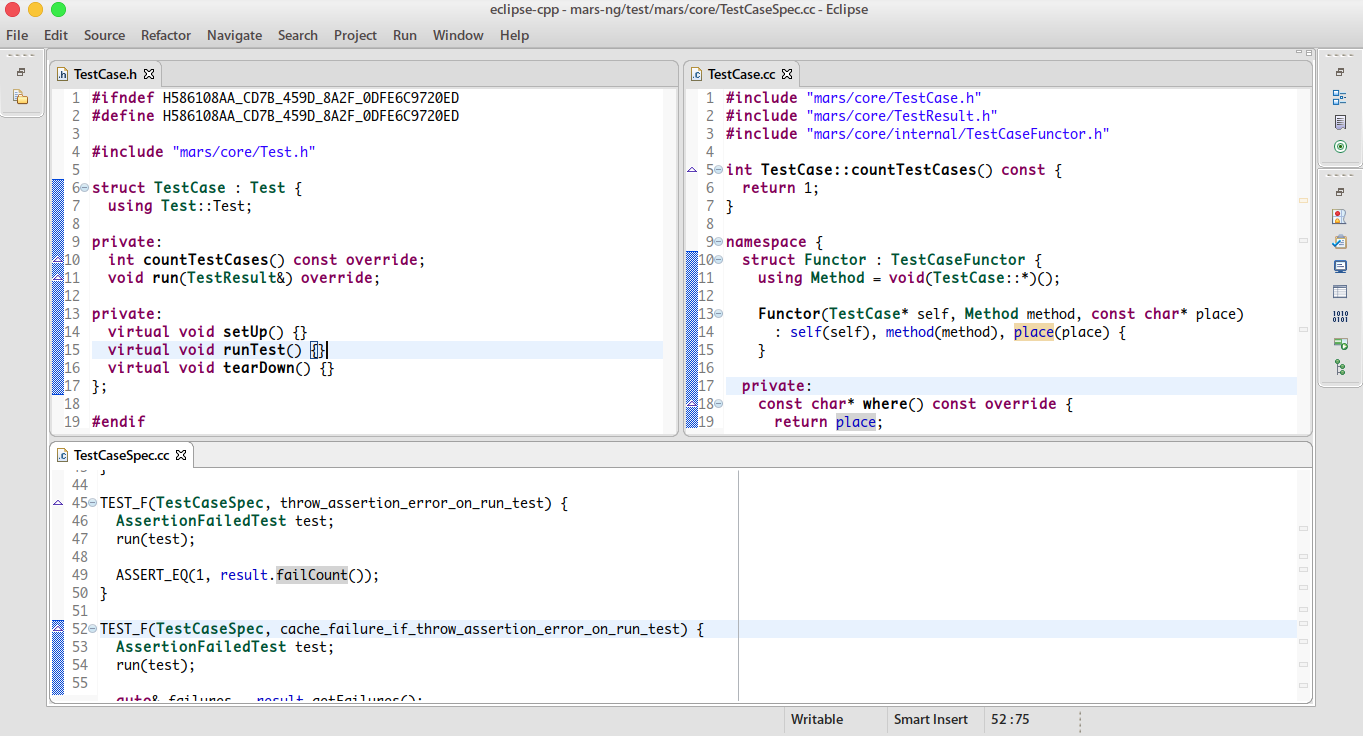
\includegraphics[width=1.0\textwidth]{figures/xunit/multi-editor-eclipse.png}
\caption{Eclipse CDT: 多屏显示}
 \label{fig:multi-editor-eclipse}
\end{figure}

因此,推荐购置高清,大屏显示器,有效改善编程环境,从而提高工作效率。此外,推荐关闭其他无关的\ascii{Tab}页,只打开当前相关的源文件,最小化外部干扰;一则让\ascii{IDE}运行速度最佳,二则使用诸如\ascii{Ctrl + E}快捷键切换文件时,最小化文件列表长度。

强烈推荐使用快捷键的优秀实践,可以成倍地提高编程的效率。例如,使用快捷键\ascii{Ctrl + Tab},在头文件与实现文件间切换自如。

\end{content}

\end{episode}

\subsection{通过测试}

在\ascii{build}临时目录中,使用\ascii{cmake}构建工程。

\begin{leftbar}
 \begin{c++}[caption={\ttfamily{构建工程}}]
$ mkdir -p build && cd build
$ cmake ..
$ make
 \end{c++}
\end{leftbar}

运行测试。

\begin{leftbar}
 \begin{c++}[caption={\ttfamily{运行测试}}]
$ test/mars-test
Running main() from gtest_main.cc
[==========] Running 1 test from 1 test case.
[----------] Global test environment set-up.
[----------] 1 test from SimpleTest
[ RUN      ] SimpleTest.make_sure_test_case_can_run_normally
[       OK ] SimpleTest.make_sure_test_case_can_run_normally (0 ms)
[----------] 1 test from SimpleTest (0 ms total)

[----------] Global test environment tear-down
[==========] 1 test from 1 test case ran. (0 ms total)
[  PASSED  ] 1 test.
 \end{c++}
\end{leftbar}


\begin{story}
  \begin{center}
    \inlinetitle{全局忽略模式}
  \end{center}

\begin{content}

\ascii{CMake}在临时目录\ascii{build}中完成系统构建,为了避免不经意地将\ascii{build}目录提交至\ascii{Git}库,常常需要在\ascii{.gitignore}文件中配置相应的忽略模式。

但是,为每个项目都创建一个\ascii{.gitignore}文件,显然是一种重复设计。因此,配置全局忽略模式是一个更恰当的解决方案。例如,在我的系统中配置如下。

\begin{leftbar}
 \begin{c++}[caption={\ttfamily{Git:配置全局忽略模式}}]
$ git config --global core.excludesfile ~/.gitignore_global
$ vi ~/.gitignore_global
# cmake
build/

# vi
*.swp

# eclipse
.project
.cproject
.settings/

# tex
output/
 \end{c++}
\end{leftbar}

\end{content}

\end{story}

\subsection{提交代码}

每当通过测试后,立即提交代码到\ascii{Git}库。

\begin{leftbar}
 \begin{c++}[caption={\ttfamily{提交代码}}]
$ git add -A .
$ git commit -m"pass first test case"
 \end{c++}
\end{leftbar}

\begin{story}
  \begin{center}
    \inlinetitle{后悔药}
  \end{center}

\begin{content}

感谢\ascii{Linus}创造了\ascii{Linux}与\ascii{Git},让全世界的程序员得以享受编程的快乐。\ascii{TDD}精髓之一便是“小”,配合运用\ascii{Git},简直就是完美,避免不经意的错误而丢失代码。

养成经常性提交代码至\ascii{Git}库,是一种良好的编程习惯。在\ascii{TDD}的一个迭代循环中,每当编译通过,链接通过,测试通过,完成重构等关键环节,都立即执行\ascii{git add}。当设计重构至相对合理状态,执行\ascii{git commit}入库。在任何时刻,都可回溯至上一个稳定的状态。如\refig{tdd-git}所示。

借助于\ascii{Git},随时可以吃后悔药。当尝试某种重构设计时,没有达到预期效果,则可以轻松回到上一个稳定状态,开始尝试新的努力。

\begin{figure}[H]
\centering
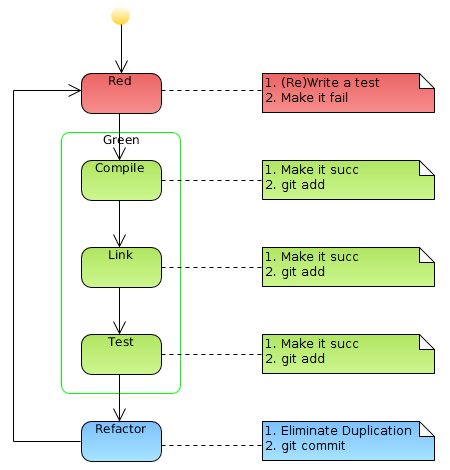
\includegraphics[width=0.6\textwidth]{figures/xunit/tdd-git.png}
\caption{TDD环: 关键环节提交代码}
 \label{fig:tdd-git}
\end{figure}

\end{content}

\end{story}

\end{content}

